\documentclass[tikz,border=3.14pt]{standalone}
\makeatletter%
\tikzset{%
  rel/.code={%
    \pgfsetlinetofirstplotpoint%
    \edef\rel@curr@x{\the\tikz@lastx}%
    \edef\rel@curr@y{\the\tikz@lasty}%
    \let\orig@tikz@plot@expression=\tikz@plot@expression%
    \def\tikz@plot@expression(##1){%
      \orig@tikz@plot@expression([shift={(\rel@curr@x,\rel@curr@y)}] ##1)%
    }
  }
}
\makeatother
\begin{document}
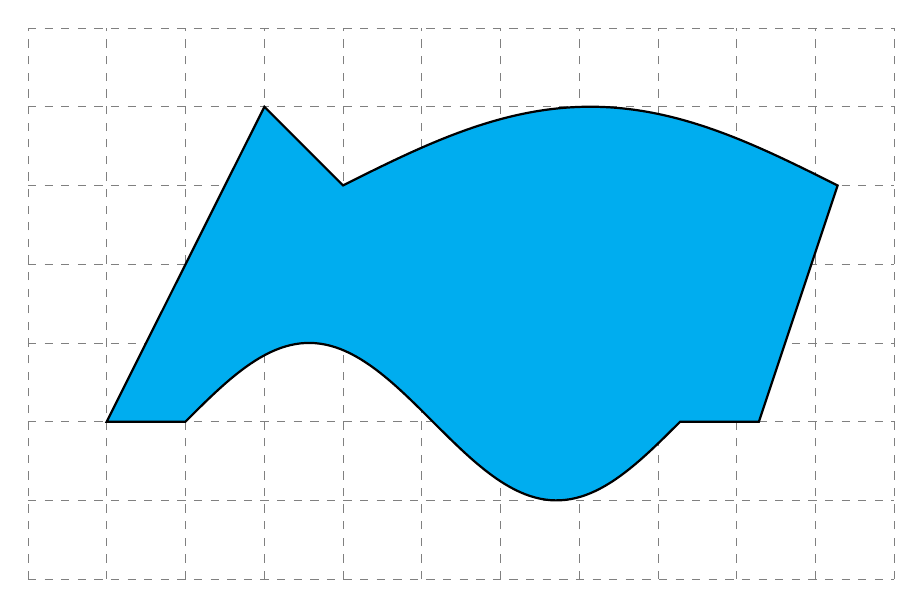
\begin{tikzpicture}[trig format=rad]
\draw[help lines,dashed] (-1,-1) grid (10,6);
\draw[thick,fill=cyan]
    (0,1) -- ++(1,0) 
    plot[rel,domain=0:2*pi,samples=100] (\x,{sin(\x)}) 
    -- ++(1,0)
    -- ++(1,3) 
    plot[rel,domain=0:pi,samples=100] (-2*\x,{sin(\x)})
    plot[rel,domain=0:1,samples=100] (-\x,\x) 
    -- cycle
;
\end{tikzpicture}
\end{document}
